\begin{problem}
Find an example of a finitely generated ring extension $R\subset
S$ where $S$ is a Noetherian ring, but $R$ is not.
\end{problem}
\begin{proof}
Let $k$ be a field and consider its polynomial ring $k[X,Y]$ in
two variables. Then we claim that the subring
$k[XY,XY^2,...]$ is non-Noetherian but its extension to
$k[X,Y]$ (by adjoining the indeterminants $X$ and $Y$)
is Noetherian by Hilbert's basis theorem. Consider the increasing
chain of ideals
\[
(XY)\subsetneq (XY,XY^2)\subsetneq(XY,XY^2,XY^3)\subsetneq\cdots.
\]
This chain does not stabilize for suppose that it did, then for
some positive integer $n$, we have
$(XY,XY^2,...,XY^n)=(XY,XY^2,...,XY^n,XY^{n+1})$ so
$XY^{n+1}\in(XY,XY^2,...,XY^n)$. But this implies that
$XY^{n+1}=p(XY,XY^2,...)q(XY,...,XY^n)$ for some polynomials $q\in
k[XY,XY^2,...]$, $q\in(XY,...,XY^n)$. Thus, we have that
\begin{align*}
\deg_Y(XY^{n+1})
&=n+1
&\deg_X(XY^{n+1})
&=1
\\
&=\deg_Y p+\deg_Y q
&&=\deg_X p+\deg_X q.
\end{align*}
Since $\deg_Y q\leq n$, $\deg_Y p\geq 1$. Thus, $\deg_X p=1$ so
$q\in k$, i.e., $q$ is a unit. This is a contradiction since
$(XY,...,XY^n)$ is a proper ideal.
\end{proof}
\newpage
\begin{problem}
Consider the homomorphism of rings
\begin{center}
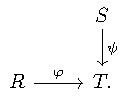
\includegraphics{figures/hw-4-ring-maps}
\end{center}
The \emph{fiber product} of $R$ and $S$ over $T$ is the subring
$R\times_T S=\left\{\,(r,s)\;\middle|\;\phi(t)=\psi(s)\,\right\}$
of $R\times S$. Assume $\phi$ and $\psi$ are surjective. Show
that if $R$ and $S$ are Noetherian rings then so is $R\times_T
S$.
\end{problem}
\begin{proof}
\begin{center}
We first prove the following result:
\begin{lemma*}[Matsumura, Ex.\,3.1]
Let $\mathfrak{a}_1,...,\mathfrak{a}_n$ be ideals of a ring $A$
such that $\mathfrak{a}_1\cap\cdots\cap\mathfrak{a}_n=0$. If each
$A/\mathfrak{a}_i$ is a Noetherian ring then so is $A$.
\end{lemma*}
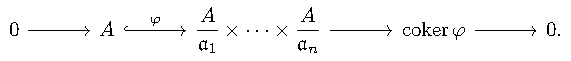
\includegraphics{figures/ps4-p2-short-exact-seq}
\end{center}
\end{proof}
\newpage
\begin{problem}
Let $M$ be an $R$-module. Show that $M$ is a flat $R$-module if
and only if $M_{\mathfrak{m}}$ is a flat
$R_{\mathfrak{m}}$-module for every maximal ideal $\mathfrak{m}$
of $R$.
\end{problem}
\begin{proof}
$\implies$
\end{proof}
\newpage
\begin{problem}
Let $M$ be an $R$-module and $\mathfrak{a}$ an $R$-ideal.
\begin{enumerate}[noitemsep,label=(\alph*)]
\item Show that if $M_{\mathfrak{m}}=0$ for every maximal ideal
  $\mathfrak{m}$ containing $\mathfrak{a}$, then $M=\mathfrak{a}M$.
\item Show that the converse holds in case $M$ is finite.
\end{enumerate}
\end{problem}
\begin{proof}
(a) Suppose that $M_{\mathfrak{m}}$ for every maximal ideal
$\mathfrak{m}$ containing $\mathfrak{a}$.
\end{proof}
\newpage
\begin{problem}
Prove that every power of a maximal ideal is primary.
\end{problem}
\begin{proof}
\end{proof}
\newpage
\begin{problem}
\begin{enumerate}[noitemsep,label=(\alph*)]
\item Show that the radical of a primary ideal is prime.
\item Find an example of a power of a prime ideal that is not
  primary.
\item Let $\mathfrak{p}$ be a prime ideal of a ring $R$ and
  $n\in\NN$. The $R$-ideal
  $\mathfrak{p}^{(n)}=R\cap\mathfrak{p}^nR_{\mathfrak{p}}$ s
  called the \emph{$n$th symbolic power of $\mathfrak{p}$}. Show
  that $\mathfrak{p}^{(n)}$ is primary.
\end{enumerate}
\end{problem}
\begin{proof}
\end{proof}

%%% Local Variables:
%%% mode: latex
%%% TeX-master: "../MA557-HW-Current"
%%% End:
